\documentclass[journal,sort]{IEEEtran}

\usepackage{lineno,hyperref}
\usepackage{bm}
\usepackage{cancel}
\usepackage{booktabs}
\usepackage{multirow}
\usepackage{array,chngpage}
\usepackage{subfigure}
\usepackage{amssymb}
\usepackage{graphicx}
\usepackage{amsmath}
\usepackage{bm}
\usepackage{diagbox}
\usepackage{cite}
\usepackage{threeparttable}
\usepackage{url}
\usepackage{setspace}
\usepackage{caption}
\DeclareMathOperator*{\argmax}{argmax}
\usepackage[linewidth=1pt]{mdframed}
\usepackage{lipsum}
\usepackage{booktabs}
\usepackage{color}
\usepackage{longtable}
\usepackage{algorithm}


\bibliographystyle{IEEEtran}

\begin{document}

\title{Adaptive and Generative Intra-frame Steganography in HEVC Video Using the Intra Block Partitioning Structure}
\author{XXXX}
	

\maketitle

\begin{abstract}
Intra-frame steganography in HEVC video is a challenge task in the field of video steganography.In this paper, steganographic characteristic of HEVC intra block partitioning structure is first analyzed. It is proved that visual quality of stego video tends to become nearly unchanged after modifying intra block partitioning structure, but the coding efficiency and security of stego video will decrease to some extent.
Based on this property, a novel steganography method based on intra block partitioning structure is proposed to embed the secret payload. In the proposed method, the secret message is not embedded into videos by modifying the cover, but is utilized to generate the cover by a generator. The cover generator can generate four different kinds of intra block partitioning structure with different depth to make full use of HEVC intra-coding structure for high-efficient video steganography.To minimize the potiential statistical detectability, an adaptive matching scheme is designed to use the appropriate generated cover for different video content.
The proposed method is examined on HD video database with different resolution and video contents,and results are further compared with previous Intra-frame steganography method to confirm the effectiveness and advantages of this method. Results also prove that compared to the traditional intra-frame cover, the intra prediction modes, the intra block partitioning structure is a more efficient and secured intra-frame hidden cover for HEVC video.


	
	
\end{abstract}	
\begin{IEEEkeywords}
		video steganography, HEVC, block partitioning structure, generative steganography
\end{IEEEkeywords}
	
\section{Introduction\label{intro}}

As an important method to ensure communication security in the network environment, Steganography has always been a key, cutting-edge research area. Steganography utilizes the characteristics of massive data exchange in the Internet, constructs a hidden channel that humans cannot detect, and transmits a large amount of secret information. This technology is both a new opportunity and a new challenge for the security communication.


One of the most challenge research task in steganography is video steganography. As a carrier of large capacity, high concealment, redundant space diversity and robustness, video has more theoretical research significance and value than image and audio steganography. Taking HEVC coded video as an example, the coding standard designed for high-definition video, the amount of data of high-definition video itself is huge, and its coding technology also brings a new coding domain steganography space, in technical complexity, algorithm security and hidden The diversity of write space is more suitable for security information steganography.

Many works have been done in both H.264/AVC and HEVC [3, 4]. Hu et al. [5] proposed a steganographic algorithm based on intra prediction mode in H.264/AVC. Yang et al. [6] have improved Hu’s method by matrix coding. Bou-chama [7] divided the intra prediction modes in H.264/AVC into four groups ac-cording to their prediction direction, the result shows a better video quality while ensuring high capacity. Zhang et al. [8] analyzed the texture of the video, and pro-posed a high security adaptive embedding algorithm using STC. Wang et al. [9] proposed intra prediction mode based method for HEVC, a mapping between an-gle difference and secret message was established to embed data. Dong et al. [10] further proposed the prediction mode steganography technology under the HEVC standard, and made a breakthrough in the capacity limitation of the previous HEVC intra prediction mode based algorithm, while also improving the security.

The contribution of  this paper including:1) a novel cover generator is proposed to 


The rest of this paper is organized as follows: In Section
2, the Steganographic characteristic of HEVC intra quadtree partition structure is described. In Section 3, the
The proposed Steganographic method for HEVC incluing the cover geneator and the mathing scheme is presented.
Section 4 gives the framework of the proposed method. Section 5 describes the experiments and results analysis for
HEVC videos. Section 5 draws the conclusion.
\section{Steganographic characteristic of Intra Block Partitioning Structure in HEVC}
In this section, the HEVC intra block partitioning structure will be first described, with which distortion analysis of visual quality, coding efficiency and security in HEVC intra steganographic algorithm can be thoroughly introduced next.
\subsection{Intra Block Partitioning Structure in HEVC }
As in all prior ITU-T and ISO/IEC JTC 1 video coding
standards since H.261, the HEVC design follows the
classic block-based hybrid video coding approach. The basic source-coding algorithm is a hybrid
of interpicture prediction to exploit temporal statistical dependences,
intrapicture prediction to exploit spatial statistical
dependences, and transform coding of the prediction residual
signals to further exploit spatial statistical dependences[].Compared with the previous coding standards, HEVC proposes and adopts some new coding technologies based on  the classic block-based hybrid coding approach. With the introduction of these new technologies, the coding efficiency of HEVC has been greatly improved. The intra quadtree block partitioning structure is one of these key technologies.


\begin{figure}[htbp!]
	\centering
	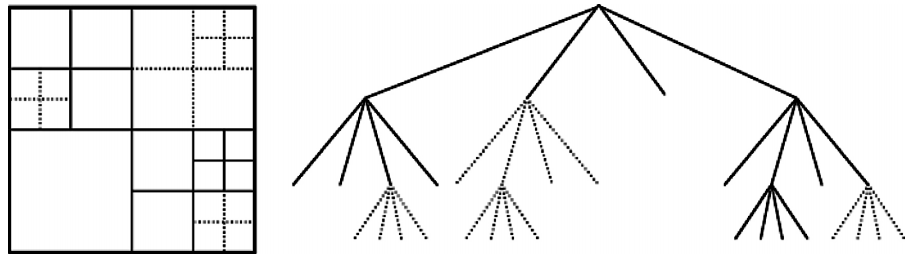
\includegraphics[width=0.5\textwidth]{1.png}
	\caption{HEVC intra partitioning structure}
	\label{HEVC-part}
\end{figure}
The HEVC standard has adopted a highly flexible and efficient block partitioning structure. Frames are splited into an integer multiple of CTU, which is an analogous term to the macroblock in H.264/AVC. A CTU consists of one luminance CTB and two chrominance CTB.The terms coding
tree block (CTB) is defined to specify the 2-D sample array of one color component associated with the CTU. In the CTU, a quadtree is established. Let CTU size be 2N$\times$2N where N is one of the values of 32, 16, or 8. The CTU can be further recursively split into four smaller units of equal sizes of N$\times$N, which are nodes of the quadtree. If the
units are leaf nodes of the quadtree, the units become coding units (CUs).

\begin{figure}[htbp!]
	\centering
	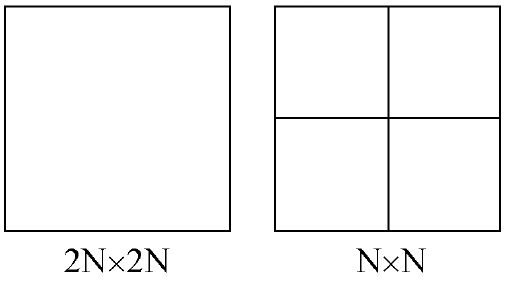
\includegraphics[width=0.2\textwidth]{2.png}
	\caption{HEVC intra partitioning structure}
	\label{HEVC-part}
\end{figure}

HEVC utilizes CU as a unit to specify which prediction
scheme is used for intra and inter predictions. One or more PUs are specified for each CU, which is
a leaf node of coding tree. Coupled with the CU, the PU
works as a basic representative block for sharing the prediction
information.A CU can be split into one, two or four PUs according to
the PU splitting type. HEVC defines two splitting shapes for
the intra coded CU.Similar to prior standards, each CU
in HEVC can be classified into three categories: skipped CU,
inter coded CU, and intra coded CU.For the intra coded CU, two possible
PU splitting types of PART2N$\times$2N and PARTN$\times$N
are supported.

The TU is the basic unit of transform and quantization, and the transform tree is a quadtree composed of transform units. Starting from the CU size, the transform unit is equally divided in an iterative manner, and whether it is divided into four sub-blocks is calibrated according to the syntax element split transform flag. The size may be one of 32$\times$32, 16$\times$16, 8$\times$8, and 4$\times$4 depending on the depth of the iteration partition.





In order to hide secret message into intra block partitionning modes, it must be clear that
how PU partitioning mode of HEVC is selected


Although use of a quadtree structure in video compression is not a new concept, the coding tree approach in HEVC can bring additional coding efficiency benefits by incorporating PU and TU quadtree concepts for video compression.




\subsection{Distortion Analysis on visual quality}
According to the HEVC intra coding scheme, this subsection will present the analysis of visual quality degradation caused by HEVC steganography, in order to illustrate the reason why large-sized PBs can be modified without introducing significant visual distortion.
Spatial-domain intra prediction has previously been successfully used in H.264/ AVC. The intra prediction of HEVC operates similarly in the spatial domain, but is extended significantly—compared to the eight prediction directions of H.264/AVC, HEVC supports a total of 33 angular prediction directions with DC and Planar mode.

\subsection{Distortion Analysis on coding efficiency}
\subsection{Distortion Analysis on Security}
\section{The proposed Steganographic method for HEVC}

\subsection{The cover generator}

\subsection{The adaptive matching scheme}
\section{Framework}



\section{Experimental results}
\section{conclusion}




	
	
	
	
	
	
	
\end{document}